%\subsection{Updated Byrd ice core chronology}\label{agedepthresults}
%\textbf{The 5,000-year accumulation function gives the best fit of the volcanic observations at the Byrd ice core, so it is used in the final ice flow model effort. The resulting uncertainties in radar depth and age to each of the layers of interest in shown in Table~\ref{tab:depthunc}. For the deepest observed reflector that can be traced between WAIS Divide ice core and Byrd ice core, the depth and age uncertainty are 0.3\% and 5\%, respectively, at the 1$\sigma$ level. The mean and median ages and depths are consistent due to the gaussian nature of the errors, as shown in Figure~\ref{fig:layer_agedepth}.}

The age-depth distribution derived for the Byrd ice core site using these methods is shown in Figure~\ref{fig:spaghetti}. This updated chronology has been trained on previously-derived ECM estimates of volcanic events observed in the Byrd ice core, but also includes estimates of uncertainty in this data, radar observations, local ice flow parameters, and local accumulation rate. 

Corresponding probability density functions generated by the metropolis algorithm sample uncertainty in the age and depth for each of four radar reflectors observed near the Byrd ice core. The age of the observed reflectors increases dramatically with depth.  These observed reflectors span to before the Last Glacial Maximum, with the oldest and deepest observed reflector dated to 25.7 $\pm$ 1.82 ka. 

We assume radar reflectors to be isochronous such that their age should be the same whether observed at the Byrd ice core or the WAIS Divide ice core. To compare between the two ice cores, we use Halliburton's Landmark seismic interpreation software to track radar reflectors through central WAIS via existing flight lines shown in Figure~\ref{fig:radarmap}. We confirm the ages we compute for all four reflectors at the Byrd ice core site agree to within uncertainty with the independently-derived WAIS Divide ice core chronology (Figures~\ref{fig:layer_histo}b,c and ~\ref{fig:spaghetti}).

Estimated values of the model parameters can be seen in the Appendix. As expected, estimations of the depth of the four radar reflectors at each iteration (Figure~\ref{fig:depthconvergence}) are correlated to each other because knowledge of the depth and age of each layer informs the relative depth and age of all other reflectors. While the accumulation rate as a function of depth is unrealistically variable, our method includes a regularization term which takes into account the smoothed accumulation rate profile, as shown in Figure~\ref{fig:accumdepth}. The smoothed profiles more closely resemble a climatic record, for which the accumulation rate was lower during the Last Glacial Maximum% ($\sim$ 1400 m depth)
. 

%  %\begin{table}
%  \centering
%  \caption{ Depth and age mean, median, and uncertainty for ten strong radar reflectors near Byrd Station, West Antarctica. The radar two-way travel time (TWTT) is given in column 1. }
%  \begin{tabular}{ c c c c c c c}
%  \cline{1-7}
%  \multirow{2}{*}{Reflector} & TWTT& & Depth (m) & & Age  (a)& \\   
% % %& ($\mu$s)& Mean & Median & $\sigma$ & & Mean & Median & $\sigma$ \\
%  & ($\mu$s)& Mean  & $\sigma$ & &Mean  & $\sigma$ \\
%  \cline{3-4} \cline{6-7}
%   1 & 8.44    & 537.5  &  0.8 & &1200 & 20   \\
%   2 & 9.58    & 633.1  &  6.5 & &1770 & 40   \\
%   3 & 12.54   & 880.8  &  7.4 & &2100 & 60   \\
%   4 & 17.55   & 1300.7 &  6.1 & &3510 & 150  \\
%   5 & 22.42   & 1711.9 &  4.4 & &4360 & 200  \\
% %  %6 & 11.10  & 596.9  & 596.9  & 2.3 & &5440 & 5440 & 270   \\
% %  %7 & 12.78  & 738.8  & 738.8  & 2.3 & &7120 & 7110 & 370   \\
% %  %8 & 13.02  & 759.1  & 759.1  & 2.3 & 7350 & 7340 & 390   \\
% %  %9 & 18.92  & 1257.7 & 1257.7 & 2.4 & 16220 & 16300 & 1760   \\
% %  %10& 19.02  & 1266.2 & 1266.2 & 2.3 & 16400 & 16500 & 1820  \\
% % %\cline{1-7}
%  \end{tabular}
% % \tablenotetext{a}{Footnote text here.}
% % %\captionsetup{width=.9\textwidth}

%  %\label{tab:depthunc}
% %\end{table}




\begin{figure*}[h]
%\begin{center}
\centering
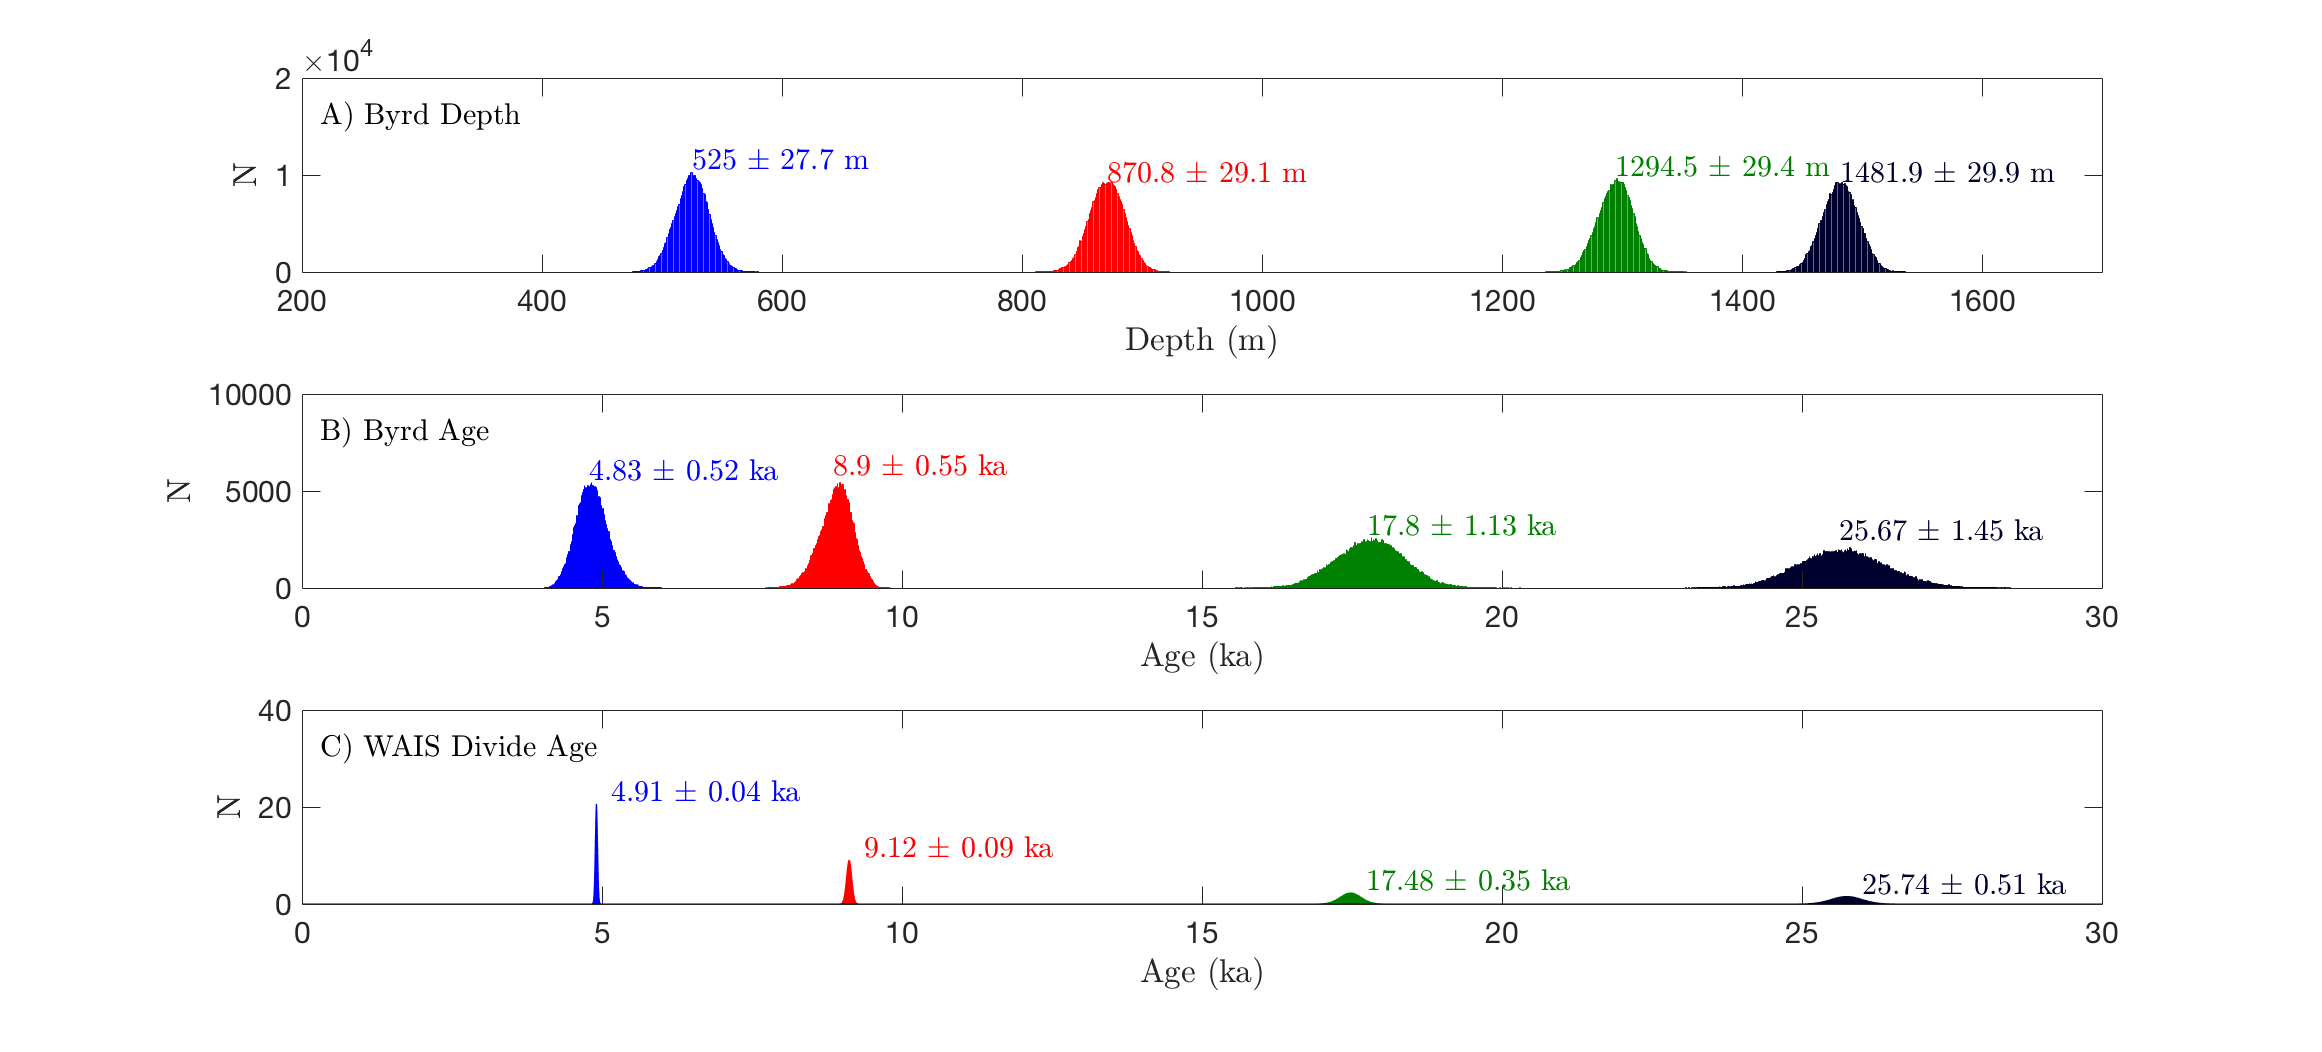
\includegraphics[scale=0.3]{../analysis/figures/agedepthhisto}
%\captionsetup{width=.9\textwidth}
\caption[]{Depth (top) and age (middle) distributions of 4 radar reflectors at the Byrd ice core and the age distribution of the same 4 reflectors at the WAIS Divide ice core (bottom). The width of the age and depth histograms for the Byrd ice core chronology represent uncertainty estimated by the methods used here. The WAIS Divide ice core distributions are recreated from the WAID Divide ice core chronology \cite{buizert2013} and are used as an independent check on our estimation of the age-depth distribution at the Byrd ice core.}
%\end{center}
\label{fig:layer_histo}
\end{figure*}

\begin{figure*}[h]
%\begin{center}
\centering
\includegraphics[scale=0.3]{../analysis/figures/spaghetti}
%\captionsetup{width=.9\textwidth}
\caption[]{Modeled age-depth relationship with uncertainty compared to measured volcanic chronology from \citet[open circles;][]{hammer97}. The WAIS Divide ice core chronogoly \citep{buizert2013} is shown in green. Blue triangles show the age-depth of 5 reflectors at each of the Byrd and WAIS Divide ice cores; these reflectors are assumed isochronous and so expected to be the same age at either ice core.}
%\end{center}
\label{fig:spaghetti}
\end{figure*}